\documentclass{article}
\usepackage{tikz}
\begin{document}
\newcommand{\key}[5]{   %Obfruscated answer 
    \fill[#5] (#2, #3) rectangle (#2+#4, #3-#4);
    \draw (#2, #3) rectangle (#2+#4, #3-#4);
    \node at (#2+#4*.5, #3-#4*.5) {#1}; %Changed these to rectangles
    }

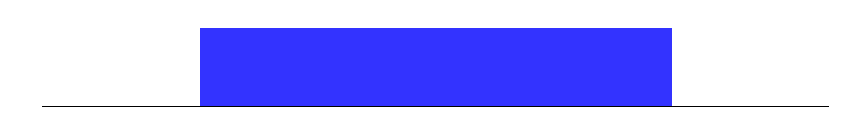
\begin{tikzpicture}
\key{`}{0}{3}{1}{blue!10};
\key{1}{1}{3}{1}{blue!0};
\key{2}{2}{3}{1}{blue!0};
\key{3}{3}{3}{1}{blue!0};
\key{4}{4}{3}{1}{blue!0};
\key{5}{5}{3}{1}{blue!0};
\key{6}{6}{3}{1}{blue!0};
\key{7}{7}{3}{1}{blue!0};
\key{8}{8}{3}{1}{blue!0};
\key{9}{9}{3}{1}{blue!0};
\key{0}{10}{3}{1}{blue!0};
\key{-}{11}{3}{1}{blue!0};
\key{=}{12}{3}{1}{blue!0};
\key{tab}{0}{2}{1}{white};
\key{q}{1}{2}{1}{blue!10};
\key{w}{2}{2}{1}{blue!0};
\key{e}{3}{2}{1}{blue!10};
\key{r}{4}{2}{1}{blue!0};
\key{t}{5}{2}{1}{blue!10};
\key{y}{6}{2}{1}{blue!0};
\key{u}{7}{2}{1}{blue!0};
\key{i}{8}{2}{1}{blue!0};
\key{o}{9}{2}{1}{blue!20};
\key{p}{10}{2}{1}{blue!0};
\key{$\backslash$}{11}{2}{1}{white};
\key{|}{12}{2}{1}{blue!0};
\key{caps}{0}{1}{1}{white};
\key{a}{1}{1}{1}{blue!100};
\key{s}{2}{1}{1}{blue!0};
\key{d}{3}{1}{1}{blue!10};
\key{f}{4}{1}{1}{blue!20};
\key{g}{5}{1}{1}{blue!0};
\key{h}{6}{1}{1}{blue!0};
\key{j}{7}{1}{1}{blue!0};
\key{k}{8}{1}{1}{blue!0};
\key{l}{9}{1}{1}{blue!0};
\key{;}{10}{1}{1}{blue!0};
\key{'}{11}{1}{1}{blue!0};
\key{enter}{12}{1}{1}{white};
\key{shift}{0}{0}{1}{white};
\key{z}{1}{0}{1}{blue!30};
\key{x}{2}{0}{1}{blue!10};
\key{c}{3}{0}{1}{blue!10};
\key{v}{4}{0}{1}{blue!0};
\key{b}{5}{0}{1}{blue!100};
\key{n}{6}{0}{1}{blue!0};
\key{m}{7}{0}{1}{blue!0};
\key{,}{8}{0}{1}{blue!0};
\key{.}{9}{0}{1}{blue!0};
\key{/}{10}{0}{1}{blue!0};
\key{?}{11}{0}{1}{blue!0};
\key{shift}{12}{0}{1}{white};

\key{ctrl}{0}{-1}{1}{red}
\key{alt}{1}{-1}{1}{red}
\key{alt}{8}{-1}{1}{red}
\key{ctrl}{9}{-1}{1}{red}
\draw (0, -2)--(10, -2);
\fill[blue!80] (2, -2) rectangle (8, -1);

\end{tikzpicture}
\end{document}
